%%%%%%%%%%%%%%%%%%%%%%%%%%%%%%%%%%%%%%%%%
% Lachaise Assignment
% LaTeX Template
% Version 1.0 (26/6/2018)
%
% This template originates from:
% http://www.LaTeXTemplates.com
%
% Authors:
% Marion Lachaise & François Févotte
% Vel (vel@LaTeXTemplates.com)
%
% License:
% CC BY-NC-SA 3.0 (http://creativecommons.org/licenses/by-nc-sa/3.0/)
% 
%%%%%%%%%%%%%%%%%%%%%%%%%%%%%%%%%%%%%%%%%

%----------------------------------------------------------------------------------------
%	PACKAGES AND OTHER DOCUMENT CONFIGURATIONS
%----------------------------------------------------------------------------------------

\documentclass{article}

%%%%%%%%%%%%%%%%%%%%%%%%%%%%%%%%%%%%%%%%%
% Lachaise Assignment
% Structure Specification File
% Version 1.0 (26/6/2018)
%
% This template originates from:
% http://www.LaTeXTemplates.com
%
% Authors:
% Marion Lachaise & François Févotte
% Vel (vel@LaTeXTemplates.com)
%
% License:
% CC BY-NC-SA 3.0 (http://creativecommons.org/licenses/by-nc-sa/3.0/)
% 
%%%%%%%%%%%%%%%%%%%%%%%%%%%%%%%%%%%%%%%%%

%----------------------------------------------------------------------------------------
%	PACKAGES AND OTHER DOCUMENT CONFIGURATIONS
%----------------------------------------------------------------------------------------

\usepackage{amsmath,amsfonts,stmaryrd,amssymb} % Math packages

\usepackage{enumerate} % Custom item numbers for enumerations

\usepackage[ruled]{algorithm2e} % Algorithms

\usepackage[framemethod=tikz]{mdframed} % Allows defining custom boxed/framed environments

\usepackage{listings} % File listings, with syntax highlighting
\lstset{
	basicstyle=\ttfamily, % Typeset listings in monospace font
}

%----------------------------------------------------------------------------------------
%	DOCUMENT MARGINS
%----------------------------------------------------------------------------------------

\usepackage{geometry} % Required for adjusting page dimensions and margins

\geometry{
	paper=a4paper, % Paper size, change to letterpaper for US letter size
	top=2.5cm, % Top margin
	bottom=3cm, % Bottom margin
	left=2.5cm, % Left margin
	right=2.5cm, % Right margin
	headheight=14pt, % Header height
	footskip=1.5cm, % Space from the bottom margin to the baseline of the footer
	headsep=1.2cm, % Space from the top margin to the baseline of the header
	%showframe, % Uncomment to show how the type block is set on the page
}

%----------------------------------------------------------------------------------------
%	FONTS
%----------------------------------------------------------------------------------------

\usepackage[utf8]{inputenc} % Required for inputting international characters
\usepackage[T1]{fontenc} % Output font encoding for international characters

\usepackage{XCharter} % Use the XCharter fonts

%----------------------------------------------------------------------------------------
%	COMMAND LINE ENVIRONMENT
%----------------------------------------------------------------------------------------

% Usage:
% \begin{commandline}
%	\begin{verbatim}
%		$ ls
%		
%		Applications	Desktop	...
%	\end{verbatim}
% \end{commandline}

\mdfdefinestyle{commandline}{
	leftmargin=10pt,
	rightmargin=10pt,
	innerleftmargin=15pt,
	middlelinecolor=black!50!white,
	middlelinewidth=2pt,
	frametitlerule=false,
	backgroundcolor=black!5!white,
	frametitle={Command Line},
	frametitlefont={\normalfont\sffamily\color{white}\hspace{-1em}},
	frametitlebackgroundcolor=black!50!white,
	nobreak,
}

% Define a custom environment for command-line snapshots
\newenvironment{commandline}{
	\medskip
	\begin{mdframed}[style=commandline]
}{
	\end{mdframed}
	\medskip
}

%----------------------------------------------------------------------------------------
%	FILE CONTENTS ENVIRONMENT
%----------------------------------------------------------------------------------------

% Usage:
% \begin{file}[optional filename, defaults to "File"]
%	File contents, for example, with a listings environment
% \end{file}

\mdfdefinestyle{file}{
	innertopmargin=1.6\baselineskip,
	innerbottommargin=0.8\baselineskip,
	topline=false, bottomline=false,
	leftline=false, rightline=false,
	leftmargin=2cm,
	rightmargin=2cm,
	singleextra={%
		\draw[fill=black!10!white](P)++(0,-1.2em)rectangle(P-|O);
		\node[anchor=north west]
		at(P-|O){\ttfamily\mdfilename};
		%
		\def\l{3em}
		\draw(O-|P)++(-\l,0)--++(\l,\l)--(P)--(P-|O)--(O)--cycle;
		\draw(O-|P)++(-\l,0)--++(0,\l)--++(\l,0);
	},
	nobreak,
}

% Define a custom environment for file contents
\newenvironment{file}[1][File]{ % Set the default filename to "File"
	\medskip
	\newcommand{\mdfilename}{#1}
	\begin{mdframed}[style=file]
}{
	\end{mdframed}
	\medskip
}

%----------------------------------------------------------------------------------------
%	NUMBERED QUESTIONS ENVIRONMENT
%----------------------------------------------------------------------------------------

% Usage:
% \begin{question}[optional title]
%	Question contents
% \end{question}

\mdfdefinestyle{question}{
	innertopmargin=1.2\baselineskip,
	innerbottommargin=0.8\baselineskip,
	roundcorner=5pt,
	nobreak,
	singleextra={%
		\draw(P-|O)node[xshift=1em,anchor=west,fill=white,draw,rounded corners=5pt]{%
		Question \theQuestion\questionTitle};
	},
}

\newcounter{Question} % Stores the current question number that gets iterated with each new question

% Define a custom environment for numbered questions
\newenvironment{question}[1][\unskip]{
	\bigskip
	\stepcounter{Question}
	\newcommand{\questionTitle}{~#1}
	\begin{mdframed}[style=question]
}{
	\end{mdframed}
	\medskip
}

%----------------------------------------------------------------------------------------
%	UNNUMBERED QUESTIONS ENVIRONMENT
%----------------------------------------------------------------------------------------

% Usage:
% \begin{question}[optional title]
%	Question contents
% \end{question}

\mdfdefinestyle{question*}{
	innertopmargin=1.2\baselineskip,
	innerbottommargin=0.8\baselineskip,
	roundcorner=5pt,
	nobreak,
	singleextra={%
		\draw(P-|O)node[xshift=1em,anchor=west,fill=white,draw,rounded corners=5pt]{%
		Question \questionTitle};
	},
}

\newcounter{Question*} % Stores the current question number that gets iterated with each new question

% Define a custom environment for unnumbered questions
\newenvironment{question*}[1][\unskip]{
	\bigskip
	% \stepcounter{Question*}
	\newcommand{\questionTitle}{~#1}
	\begin{mdframed}[style=question*]
}{
	\end{mdframed}
	\medskip
}

%----------------------------------------------------------------------------------------
%	WARNING TEXT ENVIRONMENT
%----------------------------------------------------------------------------------------

% Usage:
% \begin{warn}[optional title, defaults to "Warning:"]
%	Contents
% \end{warn}

\mdfdefinestyle{warning}{
	topline=false, bottomline=false,
	leftline=false, rightline=false,
	nobreak,
	singleextra={%
		\draw(P-|O)++(-0.5em,0)node(tmp1){};
		\draw(P-|O)++(0.5em,0)node(tmp2){};
		\fill[black,rotate around={45:(P-|O)}](tmp1)rectangle(tmp2);
		\node at(P-|O){\color{white}\scriptsize\bf !};
		\draw[very thick](P-|O)++(0,-1em)--(O);%--(O-|P);
	}
}

% Define a custom environment for warning text
\newenvironment{warn}[1][Warning:]{ % Set the default warning to "Warning:"
	\medskip
	\begin{mdframed}[style=warning]
		\noindent{\textbf{#1}}
}{
	\end{mdframed}
}

%----------------------------------------------------------------------------------------
%	INFORMATION ENVIRONMENT
%----------------------------------------------------------------------------------------

% Usage:
% \begin{info}[optional title, defaults to "Info:"]
% 	contents
% 	\end{info}

\mdfdefinestyle{info}{%
	topline=false, bottomline=false,
	leftline=false, rightline=false,
	nobreak,
	singleextra={%
		\fill[black](P-|O)circle[radius=0.4em];
		\node at(P-|O){\color{white}\scriptsize\bf i};
		\draw[very thick](P-|O)++(0,-0.8em)--(O);%--(O-|P);
	}
}

% Define a custom environment for information
\newenvironment{info}[1][Info:]{ % Set the default title to "Info:"
	\medskip
	\begin{mdframed}[style=info]
		\noindent{\textbf{#1}}
}{
	\end{mdframed}
}
 % Include the file specifying the document structure and custom commands

\usepackage{multicol}
\usepackage{graphicx}
\usepackage{caption,subcaption}
\usepackage{float}

\usepackage{array}

\usepackage{pgfplotstable}
\usepackage{booktabs}

%----------------------------------------------------------------------------------------
%	ASSIGNMENT INFORMATION
%----------------------------------------------------------------------------------------

\title{EDP1: TP1 - Problème de Poisson} % Title of the assignment

\author{Desmond Ngueguin\\ \texttt{roussel-desmond.nzoyem-ngueguin@etu.unistra.fr}} % Author name and email address

\date{Université de Strasbourg --- \today} % University, school and/or department name(s) and a date

%----------------------------------------------------------------------------------------

\begin{document}

\maketitle % Print the title

%----------------------------------------------------------------------------------------
%	INTRODUCTION
%----------------------------------------------------------------------------------------

% \section*{Introduction} % Unnumbered section

% Etude du la onvergence de la methode des elements finis appliquée a un problème de Poisson.

% \section{Verification} % Numbered section

%----------------------------------------------------------------------------------------
%	PROBLEM 1
%----------------------------------------------------------------------------------------

\section{Le Laplacien}

\begin{question}
	Création du maillage avec gmsh.
\end{question}

Voir figure 1 - (a)


\begin{question}
	Formulation variationnelle.
\end{question}

On a le problème aux limites:
\begin{equation}
	\label{eq:3}
	\begin{split}
	  -\Delta u &= 1\\
	  u &= 0\ \mbox{ sur }\ \Gamma_D\\
	  \frac{\partial u}{\partial n} &= 0\ \mbox{ sur }\ \Gamma_N\\
	  u + \frac{\partial u}{\partial n} &= 0\ \mbox{ sur }\ \Gamma_F\\
	\end{split}
\end{equation}

Posons $V= \{ v \in H^1 \langle \Omega \rangle, v_{|\Gamma_D} = 0 \} $ . $V$ est de Hilbert car l'application $ \gamma_0 : H^1 (\Omega) \to L^2(\Gamma_D) $ est continue et linéaire d'après le théorème de la trace. $V = \gamma_0^{-1} (\{0\})$ est fermé en tant qu'image réciproque d'en fermé par une application continue. $V$ est donc un sous-espace fermé d'un Hilbert, soit un Hilbert. 

Soit $u \in H^2(\Omega) $ solution de $(1)$ et $v \in V$, on a:
% \begin{equation}
	\begin{align*}
		-\Delta u = 1 &\Rightarrow \int_{\Omega}-\Delta u\,v \, d\Omega = \int_{\Omega} v \, d\Omega \\
		&\Rightarrow -\int_{\Gamma}\frac{\partial u}{\partial n} \,v \, d\Gamma + \int_{\Omega} \nabla u \, \nabla v \,d\Omega= \int_{\Omega} v \, d\Omega &&\text{(D'apres la formule de Green)}\\
		&\Rightarrow -\int_{\Gamma_D}\frac{\partial u}{\partial n} \,v \, d\Gamma_D -\int_{\Gamma_N}\frac{\partial u}{\partial n} \,v \, d\Gamma_N  -\int_{\Gamma_F}\frac{\partial u}{\partial n} \,v \, d\Gamma_F + \int_{\Omega} \nabla u \, \nabla v \,d\Omega= \int_{\Omega} v \, d\Omega\\
		&\Rightarrow -\int_{\Gamma_F}(-u) \,v \, d\Gamma_F + \int_{\Omega} \nabla u \, \nabla v \,d\Omega= \int_{\Omega} v \, d\Omega &&\text{(Car $v|_{\Gamma_D} = 0$, et d'après (1))}\\
		&\Rightarrow a(u, v) = l(v) \\
	\end{align*}
% \end{equation}
\text{avec} \,
% \begin{equation}
	\begin{align*}
			&a(u, v) = \int_{\Gamma_F}u \,v \, d\Gamma_F + \int_{\Omega} \nabla u \, \nabla v \,d\Omega \\
			&l(v) = \int_{\Omega} v \, d\Omega  && \forall \, v \in V = \{ v \in H^1 \langle \Omega \rangle, v_{|\Gamma_D} = 0 \}
	\end{align*}
% \end{equation}

Le maillage et la solution sont représentés à la figure 1:
\begin{figure}[H]
    \centering
    \begin{subfigure}[b]{0.52\linewidth}        %% or \columnwidth
        \centering
        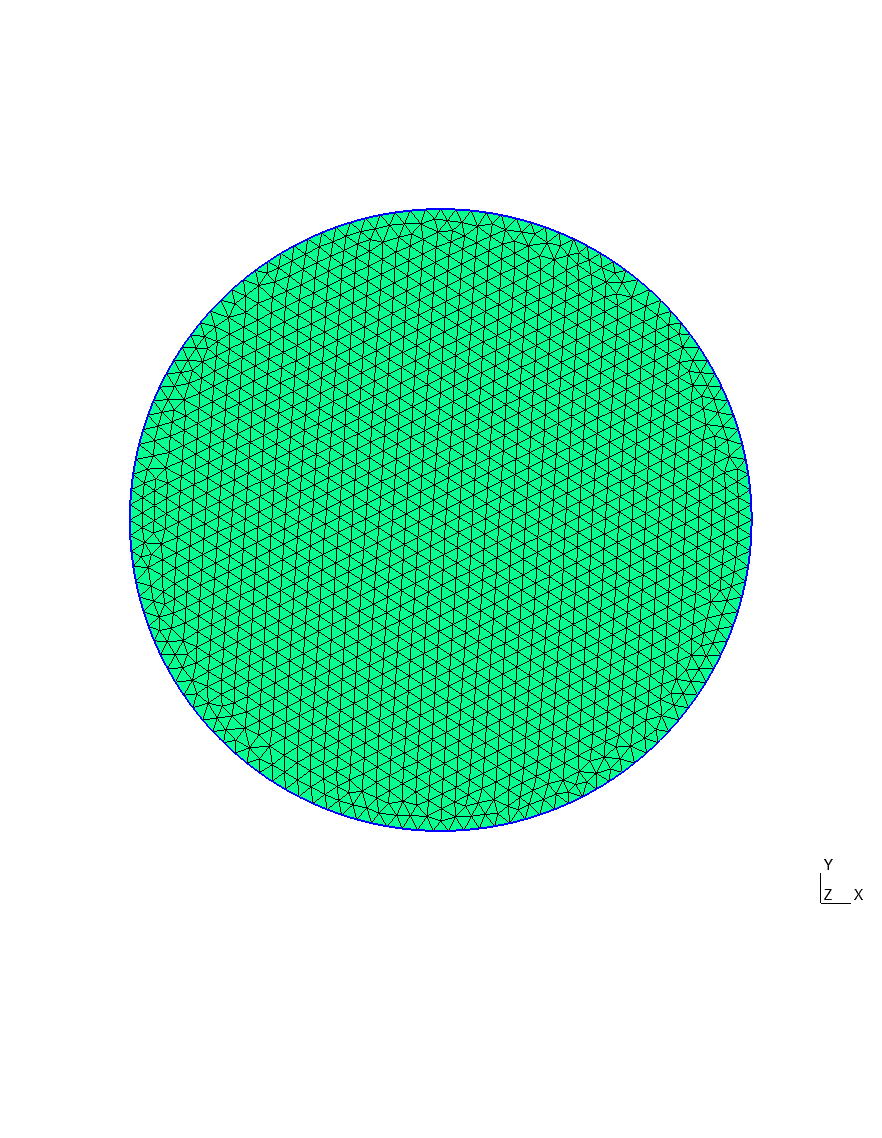
\includegraphics[width=\linewidth]{data/maillage_gmsh.png}
        \caption{Maillage Omega avec GMSH}
        \label{fig:A}
    \end{subfigure}
    \begin{subfigure}[b]{0.46\linewidth}        %% or \columnwidth
        \centering
        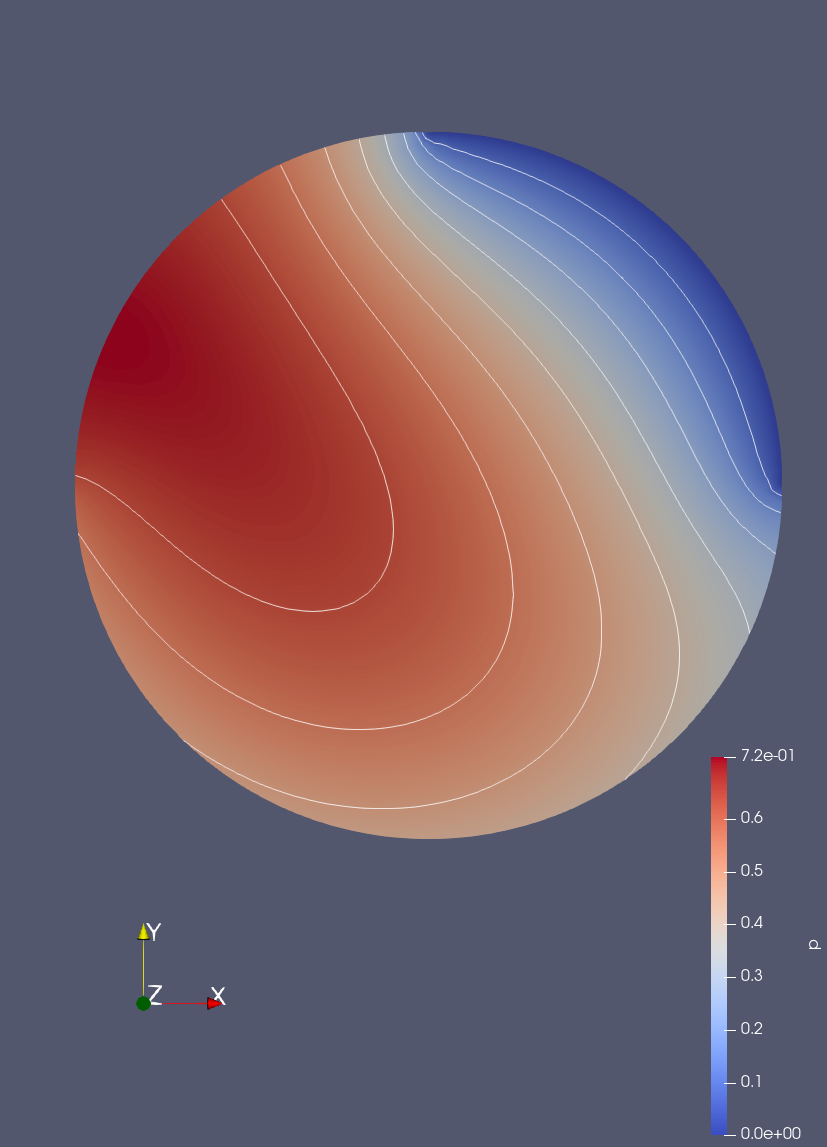
\includegraphics[width=\linewidth]{data/sol_u_lignes_de_niveau.png}
        \caption{Solution $u$ du problème avec les lignes de niveaux}
        \label{fig:B}
    \end{subfigure}
    \caption{Maillage et Solution}
    \label{fig:roc_curve}
\end{figure}


\begin{question}
	Étude de convergence avec $ u(x,y)=\sin(\pi x) \cos(\pi y) $
\end{question}

Avec la logiciel $feelpp\_qs\_laplacian$, on obtient les résultats suivant:

\begin{align*}
	&f(x,y) = 2\pi^2\sin(\pi x) \cos(\pi y) \\
	&g(x,y) = \sin(\pi x) \cos(\pi y)\\
	&m(x,y) = \pi \cos(\pi x) \cos(\pi y) - \pi \sin(\pi x) \sin(\pi y)\\
	&l(x,y) = \pi \cos(\pi x) \cos(\pi y) - \pi \sin(\pi x) \sin(\pi y) + \sin(\pi x) cos(\pi y)\\
\end{align*}


Les erreurs en normes sont présentées dans le tableau 1.


\begin{table}[H]
    \centering
    \pgfplotstableread{res.dat.txt}\loadedtable
    \pgfplotstabletypeset[columns={h,error1,error2},
    columns/{h}/.style={
    column type=r,fixed, fixed zerofill,precision=3
    },
    columns/{error1}/.style={
    column name=$\|\cdot\|_{L_2}$,
    sci,sci zerofill,
    precision=2},
    columns/{error2}/.style={
    column name=$\|\cdot\|_{H_1}$,
    sci,sci zerofill,
    precision=2},
    every head row/.style={before row=\toprule,after row=\midrule},
    every last row/.style={after row=\bottomrule}
    ]\loadedtable
    \caption{Erreur de convergence}
    \label{tab:1}
\end{table}

\begin{figure}[H]
	\centering
	\begin{tikzpicture}[scale=0.70]
		\begin{loglogaxis}[%x=3cm,
		xlabel=h,ylabel=$\|u-u_h\|$,
		% title={ error curves },
		legend style={at={(0,1)}, anchor=north west}]
		\addplot table[x=h,y={create col/linear regression={y=error1}}]{res.dat.txt};
		\xdef\slopea{\pgfplotstableregressiona}
		\addlegendentry{$L_2$ pente = $\pgfmathprintnumber{2.88}$}
		\addplot table[x=h,y={create col/linear regression={y=error2}}]{res.dat.txt};
		\xdef\slopeb{\pgfplotstableregressiona}
		\addlegendentry{$H_1$ pente = $\pgfmathprintnumber{1.91}$}
		\end{loglogaxis}
	\end{tikzpicture}
	\caption{Illustration}
	\label{fig:res}
\end{figure}

Les valeurs présentées sur la figure 2 correspondent bien à celles prédîtes par le théorème 1 de la page 39. En effet, nous résolvons le problème dans $H_2$, et on remarque bien que la pente de la courbe de l'erreur en log-log est proche de 2 pour la norme $H_1$ et de 3 = 2+1 pour la norme $L_2$.
%----------------------------------------------------------------------------------------
%	PROBLEM 2
%----------------------------------------------------------------------------------------

\section{Fonction peu régulière}
\begin{question*}
	Vérifiions que le Laplacien est bien nul.
\end{question*}

Sur $\Omega=\left\{\mathbf{x}=r(\cos \theta, \sin \theta)^{T}, r \in\right.$ $\left.(0,1), \theta \in\left(0, \frac{3 \pi}{2}\right)\right\}$, on a :
\begin{align*}
	u(r,\theta) = r^{2/3}\sin(\frac{2}{3}\theta) \quad  
	&\Rightarrow \quad \frac{\partial u}{\partial r} = \frac{2}{3}r^{-1/3}\sin(\frac{2}{3}\theta) \quad \text{et } \quad \frac{\partial u}{\partial \theta} = \frac{2}{3}r^{2/3}\cos(\frac{2}{3}\theta) \\
	&\Rightarrow \quad \frac{\partial^2 u}{\partial r^2} = -\frac{2}{9}r^{-4/3}\sin(\frac{2}{3}\theta) \quad \text{et } \quad \frac{\partial^2 u}{\partial \theta^2} = -\frac{4}{9}r^{2/3}\sin(\frac{2}{3}\theta)
\end{align*}

Le Laplacien en coordonne polaires est donné par:
\begin{align*}
	\Delta u &= \frac{\partial^2 u}{\partial r^2} + \frac{1}{r}\frac{\partial u}{\partial r} + \frac{1}{r^2}\frac{\partial^2 u}{\partial \theta^2}\\
	&=-\frac{2}{9}r^{-4/3}\sin(\frac{2}{3}\theta) + \frac{1}{r}\left\{ \frac{2}{3}r^{-1/3}\sin(\frac{2}{3}\theta) \right\} + \frac{1}{r^2}\left\{ -\frac{4}{9}r^{2/3}\sin(\frac{2}{3}\theta) \right\}\\
	&=\left( -\frac{2}{9} + \frac{6}{9} -\frac{4}{9} \right)r^{-4/3}\sin(\frac{2}{3}\theta) \\
	&= 0
\end{align*}


\begin{question*}
	Montrons que $u$ est dans $H^1(\Omega)$.
\end{question*}

On a 
\begin{align*}
	\int_{\Omega} |u|^2 d\Omega = 
	&= \int_{\Omega} \left( r^{2/3}\sin(\frac{2}{3}\theta) \right)^2 (rdrd\theta) \\
	&= \int_{0}^{1}r^{2/3}dr \int_0^{3\pi/2}sin^2(\frac{2}{3}\theta)d\theta \\
	&= \frac{3}{11} \int_0^{3\pi/2}sin^2(\frac{2}{3}\theta)d\theta \quad \in \mathbb{R}
\end{align*}

Aussi, on a $ \nabla u = \left(\frac{2}{3}r^{-1/3}\sin(\frac{2}{3}\theta), \,\frac{2}{3}r^{2/3}\cos(\frac{2}{3}\theta) \right)^T $, donc:
\begin{align*}
	\int_{\Omega} |\nabla u|^2 d\Omega = 
	&= \int_{\Omega} \left( \frac{2}{3} r^{-1/3}\sin(\frac{2}{3}\theta) \right)^2 (rdrd\theta) \\
	&= \frac{4}{9} \int_{0}^{1}r^{1/3}dr \int_0^{3\pi/2}sin^2(\frac{2}{3}\theta)d\theta \\
	&= \frac{4}{9} \times \frac{3}{4} \int_0^{3\pi/2}sin^2(\frac{2}{3}\theta)d\theta \quad \in \mathbb{R}
\end{align*}
On en déduit que $ u \in H^1(\Omega)$

Suivant la courbe $ \theta = \frac{3\pi}{4} $ par exemple, on voit que $\nabla u  = \frac{2}{3} r^{-1/3}$, et $\lim_{r \to 0} |\nabla u| = +\infty$. On conclut que $u$  n'est pas bornée à l'origine.

Pour montrer que $u \notin H^2(\Omega)$, il suffit de remarquer que le $\nabla u$ n'est pas continue, donc pas dérivable au voisinage de l'origine. En effet, si $\nabla u$ était continue en $0$, on aurait $\lim_{r \to 0} |\nabla u| = 0$.


\begin{question*}
	Créons le maillage avec Gmsh.
\end{question*}

\begin{figure}[H]
    \centering
	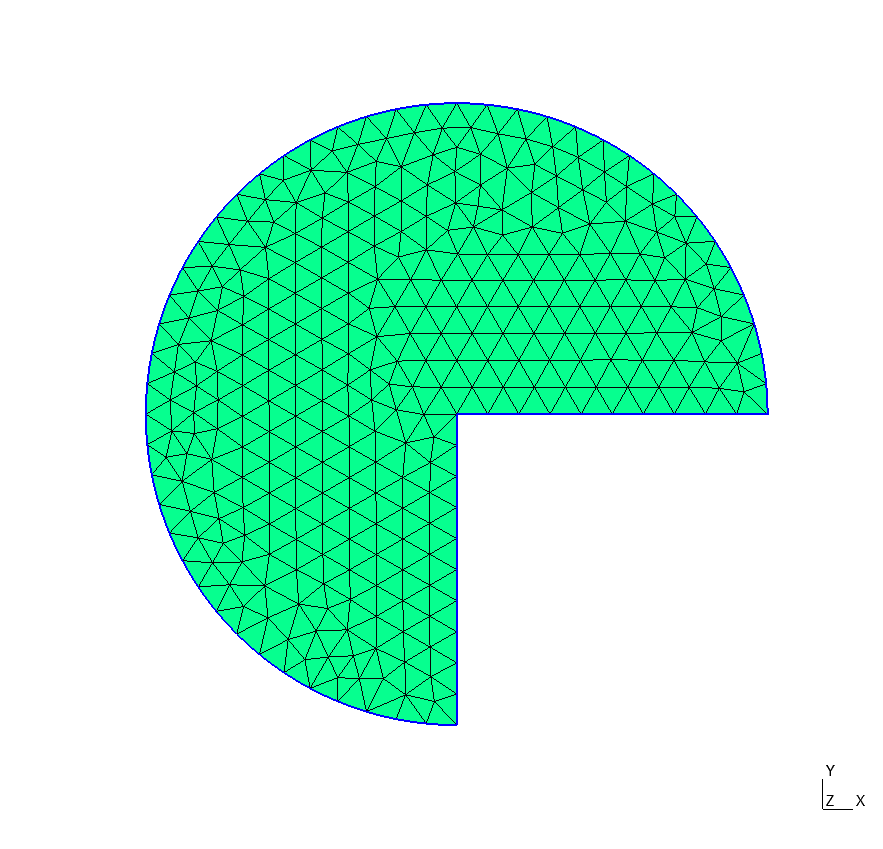
\includegraphics[width=.5\linewidth]{data/maillage_2_gmsh.png}
    \caption{Maillage avec GMSH}
    \label{fig:gmsh2}
\end{figure}

\begin{question*}
	Étude de convergence.
\end{question*}

\begin{table}[H]
    \centering
    \pgfplotstableread{res_2.dat.txt}\loadedtable
    \pgfplotstabletypeset[columns={h,error1,error2},
    columns/{h}/.style={
    column type=r,fixed, fixed zerofill,precision=3
    },
    columns/{error1}/.style={
    column name=$\|\cdot\|_{L_2}$,
    sci,sci zerofill,
    precision=2},
    columns/{error2}/.style={
    column name=$\|\cdot\|_{H_1}$,
    sci,sci zerofill,
    precision=2},
    every head row/.style={before row=\toprule,after row=\midrule},
    every last row/.style={after row=\bottomrule}
    ]\loadedtable
    \caption{Erreur de convergence}
    \label{tab:2}
\end{table}

\begin{figure}[H]
	\centering
	\begin{tikzpicture}[scale=0.70]
		\begin{loglogaxis}[%x=3cm,
		xlabel=h,ylabel=$\|u-u_h\|$,
		% title={ error curves },
		legend style={at={(0,1)}, anchor=north west}]
		\addplot table[x=h,y={create col/linear regression={y=error1}}]{res_2.dat.txt};
		\xdef\slopea{\pgfplotstableregressiona}
		\addlegendentry{$L_2$ pente = $\pgfmathprintnumber{1.52}$}
		\addplot table[x=h,y={create col/linear regression={y=error2}}]{res_2.dat.txt};
		\xdef\slopeb{\pgfplotstableregressiona}
		\addlegendentry{$H_1$ pente = $\pgfmathprintnumber{0.61}$}
		\end{loglogaxis}
	\end{tikzpicture}
	\caption{Illustration}
	\label{fig:res2}
\end{figure}

Comme le montre la figure 4, on obtient une convergence beaucoup plus lente que dans le cas d'une solution régulière. Mais cela vérifie toujours le théorème 1 de la page 39, car la solution n'est que dans $H^1(\Omega)$, et les pentes des erreurs en norme $L^2$ et $H^1$ sont respectivement plus petites que 2=1+1 et 1 (a une constante près). 

\end{document}
